\documentclass[12pt,fleqn]{article}\usepackage{../common}
\begin{document}
Kisitli Boltzmann Makinalari (Restricted Boltzmann Machines -RBM-)

Ikisel (binary) degerler tasiyan, gizli (hidden) $h$ degiskenler, ve yine
ikisel, gorunen (visible) degiskenler $v$ vardir. $Z$ aynen once gordugumuz
Boltzman Makinalarinda oldugu gibi normalizasyon sabitidir.

$$ p(x,h;W) = \exp (-E(x,h)) / Z $$

$$ E(x,h) = -h^TWx - c^Tx - b^Th $$

$$ = - \sum_j \sum_k W_{j,k}h_jx_k - \sum_k c_kx_k - \sum_j b_jh_j  $$

Dikkat: $h,x$ degiskenleri birer rasgele degiskendir. Yani hem $x$'e hem de
$h$'e ``zar attirabiliriz'', ya da bu degiskenlerden orneklem
toplayabiliriz. Bu kritik bir konu. RBM'lerin alttaki gibi resmedildigini
gorebilirsiniz.

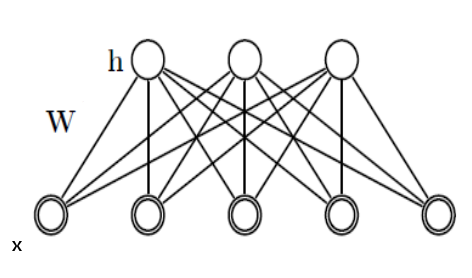
\includegraphics[height=4cm]{rbm_01.png}
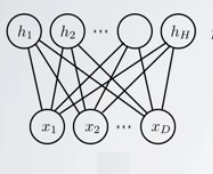
\includegraphics[height=4cm]{rbm_02.png}

Cebirsel olarak sunlar da dogrudur,

$$ p(x,h;W) = \exp (-E(x,h)) / Z $$

$$ = \exp (h^TWx + c^Tx + b^Th ) / Z $$

$$ = \exp (h^TWx) \exp (c^Tx) \exp(b^Th) / Z $$

Eger matris / vektor icindeki degerleri ayri degiskenler olarak gormek
istersek, 

$$ 
p(x,h;W) = \frac{1}{Z}
\prod_j \prod_k \exp (W_{jk}h_jx_k) \prod_k \exp(c_kx_k) \prod_j \exp(b_jh_j) 
 $$
















\end{document}
